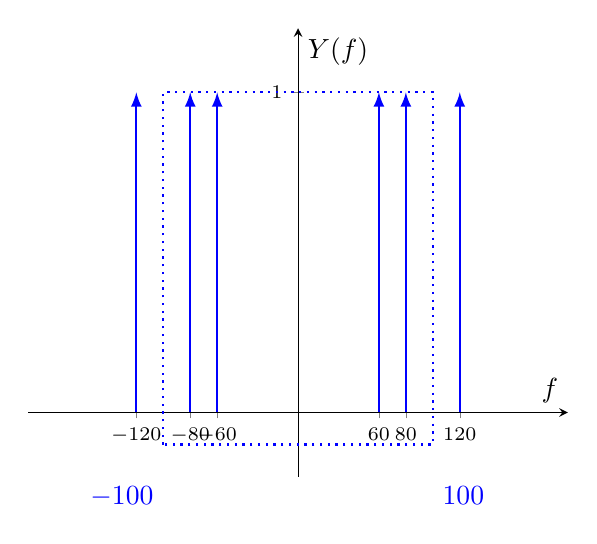
\begin{tikzpicture}
\begin{axis}[
    axis lines=middle,
    xlabel=$f$,
    ylabel=$Y(f)$,
    ymax=1,
    ymin=0,
    xmin=-200,
    xmax=200,
    xtick={ -120, -80, -60, 60, 80, 120},
    ytick={0,1},
    yticklabels={0,1},
    ticklabel style={font=\scriptsize},
    enlargelimits={abs=0.2},
    clip=false
]
% One-sided arrows
\draw[->, >=latex, blue, thick] (axis cs: -120, 0) -- (axis cs: -120, 1);
\draw[->, >=latex, blue, thick] (axis cs: -80, 0) -- (axis cs: -80, 1);
\draw[->, >=latex, blue, thick] (axis cs: -60, 0) -- (axis cs: -60, 1);
\draw[->, >=latex, blue, thick] (axis cs: 60, 0) -- (axis cs: 60, 1);
\draw[->, >=latex, blue, thick] (axis cs: 80, 0) -- (axis cs: 80, 1);
\draw[->, >=latex, blue, thick] (axis cs: 120, 0) -- (axis cs: 120, 1);
% Dotted box
\draw[blue, dotted, thick] (axis cs: -100, -0.1) rectangle (axis cs: 100, 1);
\node[blue, below right] at (axis cs: 100, -0.2) {$100$};
\node[blue, below left] at (axis cs: -100, -0.2) {$-100$};
\end{axis}
\end{tikzpicture}
